\section{گرامر زبان‌های مستقل از متن}
\subsection{}
\begin{enumerate}
    \item کافی است که کاری کنیم که سمت راست تساوی تعداد حروفش برابر با سمت چپ باشد. این کار را با
    عبارتی همچون
    $S \rightarrow LSR | \epsilon$
    انجام داد. اما مشکلی که وجود دارد این است که نمی‌توانیم که مرزی برای
    $a$ و $b$
    و
    $c$ و $d$
    تعیین کنیم. به همین جهت بر روی آن مرز حالت بندی می‌کنیم. برای همین گرامر ما به صورت زیر در می‌آید:
    \begin{align*}
        S &\rightarrow aSd ~|~ bAd ~|~ aBc ~|~ bCc ~|~ \epsilon\\
        A &\rightarrow bAd ~|~ bCc ~|~ \epsilon\\
        B &\rightarrow aBc ~|~ bCc ~|~ \epsilon\\
        C &\rightarrow bCc ~|~ \epsilon
    \end{align*}
    \item تا حدودی مثل قسمت قبل عمل می‌کنیم:
    \begin{align*}
        S &\rightarrow Ab\\
        A &\rightarrow aAa ~|~ aAb ~|~ bAa ~|~ bAb ~|~ a\\
    \end{align*}
\end{enumerate}
\subsection{}
\begin{enumerate}
    \item در ابتدا رفتار
    $S$
    را بررسی می‌کنیم. متوجه می‌شویم که خط اول عباراتی همچون
    $S\#S\#\dots$
    را تولید می‌کند. به عبارت دیگری
    $S(\#S)^*$.
    حال به جای هر کدام از
    $S$ها
    می‌توان
    $A$
    قرار داد. حال رفتار
    $A$
    را بررسی می‌کنیم. به صورت نامتناهی می‌توان در سمت چپ
    $A$، 0 قرار داد
    و در نهایت
    $A$
    را با
    \lr{10}
    جایگزاری کرد. پس زبان این عبارت برابر است با
    \begin{gather*}
        0^*10(\#0^*10)^*
    \end{gather*}
    (عملا زبان منظم بود)
    \item عملا این زبان شبیه زبان قسمت دوم قسمت قبل است. یعنی
    \begin{gather*}
        \{avu | v, u \in \{a, b\}^* \land |v| = |u|\} \cup \{bvu | v, u \in \{a, b\}^* \land |v| = |u|\}
    \end{gather*}
\end{enumerate}
\subsection{}
\begin{enumerate}
    \item به صورت زیر:
    \begin{figure}[H]
        % http://ironcreek.net/syntaxtree/
        % [S [B [A b [B b]] b] [B b]]
        % [S [B b] [B [A [B b] b] b]]
        \centering
        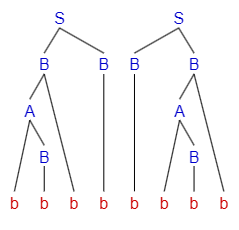
\includegraphics[scale=0.5]{pics/1-3-1.png}
    \end{figure}
    \item در ابتدا باید $S$ را از سمت راست تمامی تساوی‌ها حذف کنیم. همچنین شروع
    زبان را از
    $S_0$
    در نظر می‌گیریم.
    \begin{align*}
        S_0 &\rightarrow S\\
        S &\rightarrow ASB ~|~ BB\\
        A &\rightarrow SAa ~|~ bB ~|~ a\\
        B &\rightarrow Ab ~|~ Sa ~|~ b
    \end{align*}
    حال قوانینی اضافه می‌‌کنیم که ترمینال با متغیر قاطی نباشد.
    \begin{align*}
        S_0 &\rightarrow S\\
        S &\rightarrow ASB ~|~ BB\\
        A &\rightarrow SAN_a ~|~ N_bB ~|~ a\\
        B &\rightarrow AN_b ~|~ SN_a ~|~ b\\
        N_a &\rightarrow a\\
        N_b &\rightarrow b
    \end{align*}
    حال
    \lr{unit rule}
    $S_0 \rightarrow S$
    را حذف می‌کنیم.
    \begin{align*}
        S_0 &\rightarrow ASB ~|~ BB\\
        S &\rightarrow ASB ~|~ BB\\
        A &\rightarrow SAN_a ~|~ N_bB ~|~ a\\
        B &\rightarrow AN_b ~|~ SN_a ~|~ b\\
        N_a &\rightarrow a\\
        N_b &\rightarrow b
    \end{align*}
    در نهایت نیز متغیر‌هایی سه تایی را تبدیل به دوتایی می‌کنیم.
    \begin{align*}
        S_0 &\rightarrow AC ~|~ BB\\
        S &\rightarrow AC ~|~ BB\\
        A &\rightarrow SD ~|~ N_bB ~|~ a\\
        B &\rightarrow AN_b ~|~ SN_a ~|~ b\\
        N_a &\rightarrow a\\
        N_b &\rightarrow b\\
        C &\rightarrow SB\\
        D &\rightarrow AN_a
    \end{align*}
    \item بله. به طریق مشابه قسمت اول داریم:
    \begin{figure}[H]
        % http://ironcreek.net/syntaxtree/
        % [S_s [B [A [N_b b] [B b]] [N_b b]] [B b]]
        % [S_s [B b] [B [A [N_b b] [B b]] [N_b b]]]
        \centering
        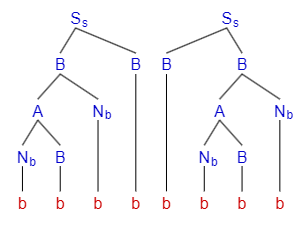
\includegraphics[scale=0.5]{pics/1-3-3.png}
    \end{figure}
\end{enumerate}